%% LyX 2.2.3 created this file.  For more info, see http://www.lyx.org/.
%% Do not edit unless you really know what you are doing.
\documentclass[english]{article}
\usepackage{lmodern}
\renewcommand{\sfdefault}{lmss}
\usepackage{courier}
\usepackage[T1]{fontenc}
\usepackage[latin1]{inputenc}
\usepackage{geometry}
\geometry{verbose,tmargin=1in,bmargin=1in,lmargin=1in,rmargin=1in,headheight=0in,headsep=0in}
\usepackage[active]{srcltx}
\usepackage{color}
\usepackage{babel}
\usepackage[unicode=true]
 {hyperref}
\usepackage{graphicx}
\makeatletter

%%%%%%%%%%%%%%%%%%%%%%%%%%%%%% LyX specific LaTeX commands.
\newcommand{\noun}[1]{\textsc{#1}}
%% Because html converters don't know tabularnewline
\providecommand{\tabularnewline}{\\}

%%%%%%%%%%%%%%%%%%%%%%%%%%%%%% Textclass specific LaTeX commands.
\newenvironment{lyxcode}
{\par\begin{list}{}{
\setlength{\rightmargin}{\leftmargin}
\setlength{\listparindent}{0pt}% needed for AMS classes
\raggedright
\setlength{\itemsep}{0pt}
\setlength{\parsep}{0pt}
\normalfont\ttfamily}%
 \item[]}
{\end{list}}

\makeatother

\begin{document}
\begin{center}
\textbf{\large{}CSCE 221 Assignment 4 Cover Page}\\
\bigskip{}
\par\end{center}

First Name~~~~~~Hunter~~~~~~Last
Name ~~~~~Cleary~~~~UIN~~625001547~~\bigskip{}

User Name ~~~hncleary~~~~~~~~~~E-mail
address~~~hncleary@tamu.edu~~~~~\medskip{}

Please list all sources in the table below including web pages which
you used to solve or implement the current homework. If you fail to
cite sources you can get a lower number of points or even zero, read
more on Aggie Honor System Office website: \texttt{\href{http://aggiehonor.tamu.edu/}{http://aggiehonor.tamu.edu/}}\medskip{}
\medskip{}
\noindent \begin{flushleft}
\begin{tabular}{|c|c|c|c|c|}
\hline 
Type of sources  & ~~~~~~~~~~~~~~~~~~~~~~~ & ~~~~~~~~~~~~~~~~~~~~~~~~ & ~~~~~~~~~~~~~~~~~~~~~~~ & ~~~~~~~~~~~~~~~~~~~~~~~\tabularnewline
 &  &  &  & \tabularnewline
\hline 
People &  &  &  & \tabularnewline
 &  &  &  & \tabularnewline
\hline 
Web pages (provide URL)  & Listed Below &  &  & \tabularnewline
 &  &  &  & \tabularnewline
\hline 
Printed material & Data Structures and Algorithms  &  &  & \tabularnewline
 &(Textbok)&  &  & \tabularnewline
\hline 
Other Sources  &  &  &  & \tabularnewline
 &  &  &  & \tabularnewline
\hline 
\end{tabular}
\par\end{flushleft}
https://www.geeksforgeeks.org/get-level-of-a-node-in-a-binary-tree/\ \\
https://www.geeksforgeeks.org/binary-search-tree-set-1-search-and-insertion/\ \\
https://www.cs.usfca.edu/~galles/visualization/BST.html\ \\
http://www.algolist.net/Data\_structures/Binary\_search\_tree/Insertion\ \\
http://www.cplusplus.com/forum/general/31509/\ \\
http://code.activestate.com/recipes/577552-binary-search-tree/\ \\
http://www.cplusplus.com/forum/beginner/75440/\ \\
http://www.cplusplus.com/reference/queue/queue/\ \\
\medskip{}
\medskip{}

\noindent I certify that I have listed all the sources that I used
to develop the solutions/codes to the submitted work.

\noindent \emph{On my honor as an Aggie, I have neither given nor
received any unauthorized help on this academic work}.

\bigskip{}
\bigskip{}

\begin{tabular}{cccccc}
Your Name  & ~~~Hunter~~~Cleary~~~~ &  & ~~~~~~~~~~~~~~~~~ & Date ~~~~ 4-1-2018 &  ~~~~~~~~~~~~~~~~~~~~\tabularnewline
\end{tabular}\pagebreak{}
\ \\


\begin{center}
\textbf{\Large{}Assignment~4 (100 pts)\medskip{}
}{\Large{}  }
\par\end{center}{\Large \par}

\begin{center}
\textbf{Program: Due April 2 at 11:59 pm }
\par\end{center}

\noindent \textbf{Objectives: Programming (70 points)}


\ \\

\textbf{Report (30 points)}


Write a brief report that includes the following:
\begin{enumerate}
\item A description of the assignment objective, how to compile and run
your programs, and an explanation of your program structure (i.e.,
a description of the classes you use, the relationship between the
classes, and the functions or classes in addition to those in the
lecture notes).\ \\
\ \\
The objective of the assignment was to create a binary search tree and then be able to calculate search costs of nodes in the structure. Two structures exist. On for the nodes within the search tree and another structure for the tree itself. The search tree contains the nodes which hold values and pointers to other nodes in the tree. The tree contains overloaded operators and functions for input and calculating search cost.
\ \\ \ \\
The program can be compiled using the make file.\ \\
Makefile\ \\
./main\ \\
\ \\
\item A brief description of the data structure you create (i.e., a theoretical
definition of the data structure and the actual data arrangement in
the classes).\ \\
\ \\
Binary search are a data structure that allows for faster access of data indexed by keys. The initial creation of the tree has a greater cost, but afterwards the cost of operations to find items in the tree is greatly reduced. Nodes traverse from root to leaf, typically using left and right subtrees. Each comparison in these subtrees allows the operations to skip an average of half the tree. Inserting and deleting items happens in logarithmic time.
\ \\
\item A description of how you implement the calculation of\textcolor{black}{{}
(a) individual search cost and (b) average search cost and explain
which tree operation (e.g. find, insert) was helpful. Analyze the
time complexity of (a) calculating individual search cost and (b)
}\textbf{summing up} the search costs over all the nodes.\ \\
\ \\
\textbf{(a)} Search cost calculation was implemented by creating a value for search cost in the search function of the binary search tree.($O(n)$)\ \\
\textbf{(b)} To calculate the average search cost, the total cost is calculated and then divided by the number of nodes present in the tree.($O(n)$)
\ \\
\item Give individual search cost in terms of \emph{$n$} using big-O notation.
Analyze and give the average search costs of a perfect binary tree
and a linear binary tree using big-O notation, assuming that the following
formulas are true (\emph{$n$} denotes the total number of integers).\ \\
$\sum_{d=0}^{\log_{2}(n+1)-1}2^{d}(d+1)\simeq(n+1)\cdot\log_{2}(n+1)-n$
~~and~~  $\sum_{d=1}^{n}d\simeq n(n+1)/2$\ \\
\ \\
Search cost of each item will be $O(logn)$. 

\textbf{Linear Tree} \ The height of the tree is n-1. Using the formula the total cost can be represented as n(n+1)/2. Dividing by n subproblems we get (n+1)/2 which is O(n).
\ \\
\ \\
\textbf{Perfect Tree} \ The height of the tree is logn. There are $2^n$ nodes at each level of the tree. $2^(log(n+1)-1)log(n+1)$ which is $O(logn)$.
\ \\
\item Include a table and a plot of average search costs you obtain. In
your discussions of the experimental results, compare the curves of
search costs with your theoretical analysis results in item 4.
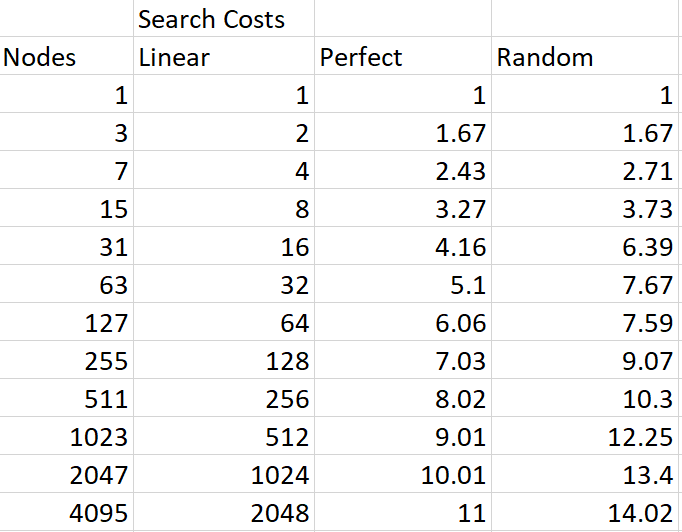
\includegraphics[width=12cm,height=\textheight,keepaspectratio]{ExcelScreen.png}\ \\
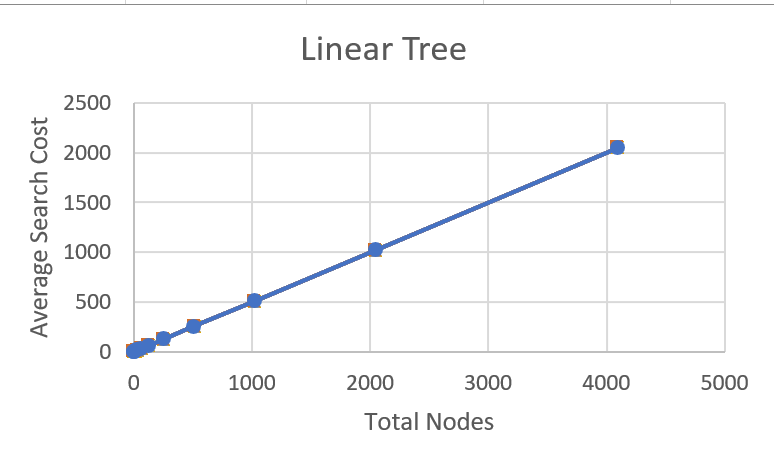
\includegraphics[width=10cm,height=\textheight,keepaspectratio]{ExcelScreen2.png}\ \\
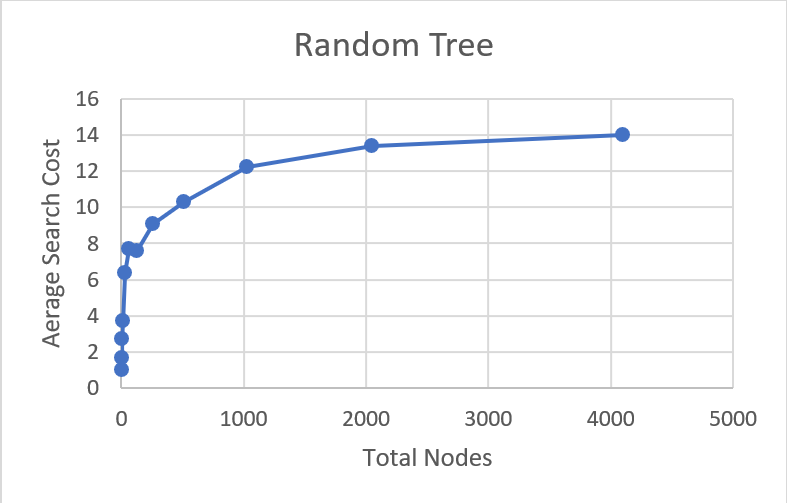
\includegraphics[width=10cm,height=\textheight,keepaspectratio]{ExcelScreen3.png}\ \\
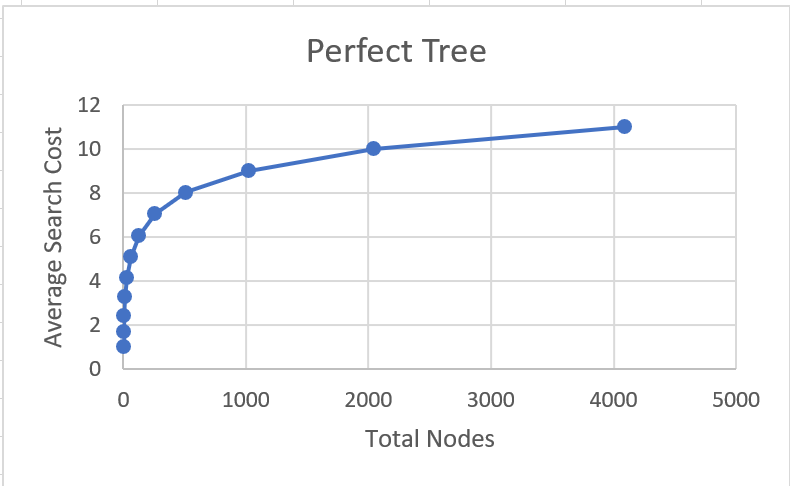
\includegraphics[width=10cm,height=\textheight,keepaspectratio]{ExcelScreen4.png}\ \\
\ \\
The experimental results were representative of the theoretical analysis. Average / random and perfect case were both $O(logn)$. Linear came out as $O(n)$.


\end{enumerate}

\end{document}
